\section{Results}
%% i.e. validation against swiss norms
\subsection{Validation}
%%Chris
To validate the externality values estimated using MATSim, the produced outputs are analyzed both temporally and spatially to check for plausibility and then compared with estimates from previous Swiss external cost reports.

\subsubsection{Emissions}
Emissions values can be estimated with MATSim directly from the processed GPS traces and therefore do not explicitely require a calibrated MATSim scenario for Switzerland.
Nevertheless, in order to validate our estimations, emission values are first calculated using a 10\% MATSim scenario for Switzerland.
To comply with new vehicle registration statistics according to \citet{autoschweiz2010}, \citet{autoschweiz2012} and \citet{energieVerbrauchEffizienzPersonenwagen2015} as well as the vehicle ownership predictions from \citet{foen2010pollutants}, two scenarios where 30\% and 40\% of vehicles are randomly assigned a diesel engine were examined.

The emission values are estimated for each road link in the MATSim network for the following pollutants: CO, total CO$_2$, FC, HC, NMHC, NO$_2$, NO$_x$, PM and SO$_2$.
The values are aggregated into hourly time bins.
These emission estimates are then first analyzed temporally and spatially to assure the plausibility of the output.

When analyzing the temporal evolution of emissions over the course of a typical workday, we would expect it to correlate with typical commuter patterns, i.e. low emissions both in the early morning and late evening and higher emissions during the day, with spikes corresponding to rush-hour periods.
\Cref{fig:hourlyEmissions} shows the typical daily emission of each pollutant per hourly time bin estimated from the MATSim scenario, for both the 30\% and 40\% diesel engine ownership scenarios.
Note that only total CO$_2$ and FC are shown, as the emissions values for the other pollutants are negligeable in comparison.
As expected, two distinct peaks corresponding to morning and evening rush-hour can be observed, while the early morning and late-night values are near zero and the midday values lie somewhere in between.

\createfigure%
{Hourly emissions values for Switzerland}%
{Hourly emissions values for Switzerland. Only total CO$_2$ and FC emissions are shown, as the values for the other pollutants are negligeable in comparison.}%
{\label{fig:hourlyEmissions}}%
{%
  \createsubfigure%
  {30\% diesel vehicles}%
  {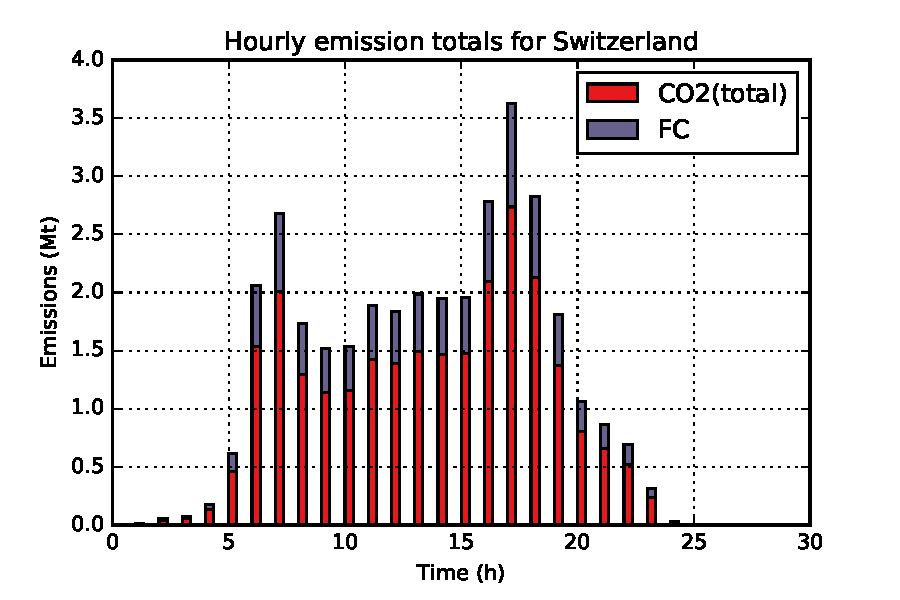
\includegraphics[width=0.49\textwidth,
angle=0]{figures/hourly_emissions_30pct_diesel.pdf}}%
  {\label{fig:hourlyEmissions-30pctDiesel}}%
  {}%
  \createsubfigure%
  {40\% diesel vehicles}%
  {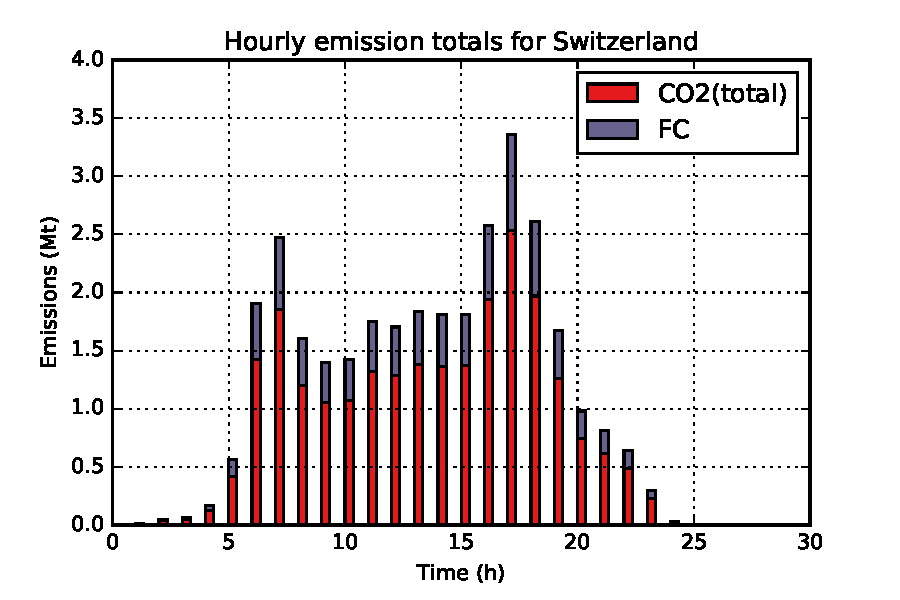
\includegraphics[width=0.49\textwidth,
angle=0]{figures/hourly_emissions_40pct_diesel.pdf}}%
  {}%
}%
{}

The spatial analysis of emissions is expected to show higher emissions in and around larger cities and within highly populated cantons, where more people live and therefore more commutes are observed.
\Cref{fig:spatialEmissions} shows the spatial distribution of the total daily emissions over all of Switzerland with 40\% diesel engine ownership.
The heatmap is generated by summing the total emissions with a 10 km radius around each point.
Indeed, it can be seen that total emission values are higher in the main metropolitan areas (Zurich, Geneva, Basel, Bern, Lausanne, Lucerne, St-Gallen) than in rural areas within e.g. Graub\"unden, Valais, Schwyz or Appenzell.
Higher emissions also tend to coincide with the presence of motorways.

\createfigure%
{Spatial distribution of total emissions in Switzerland with 40\% diesel engines}%
{Spatial distribution of total emissions in Switzerland with 40\% diesel engines}%
{\label{fig:spatialEmissions}}%
{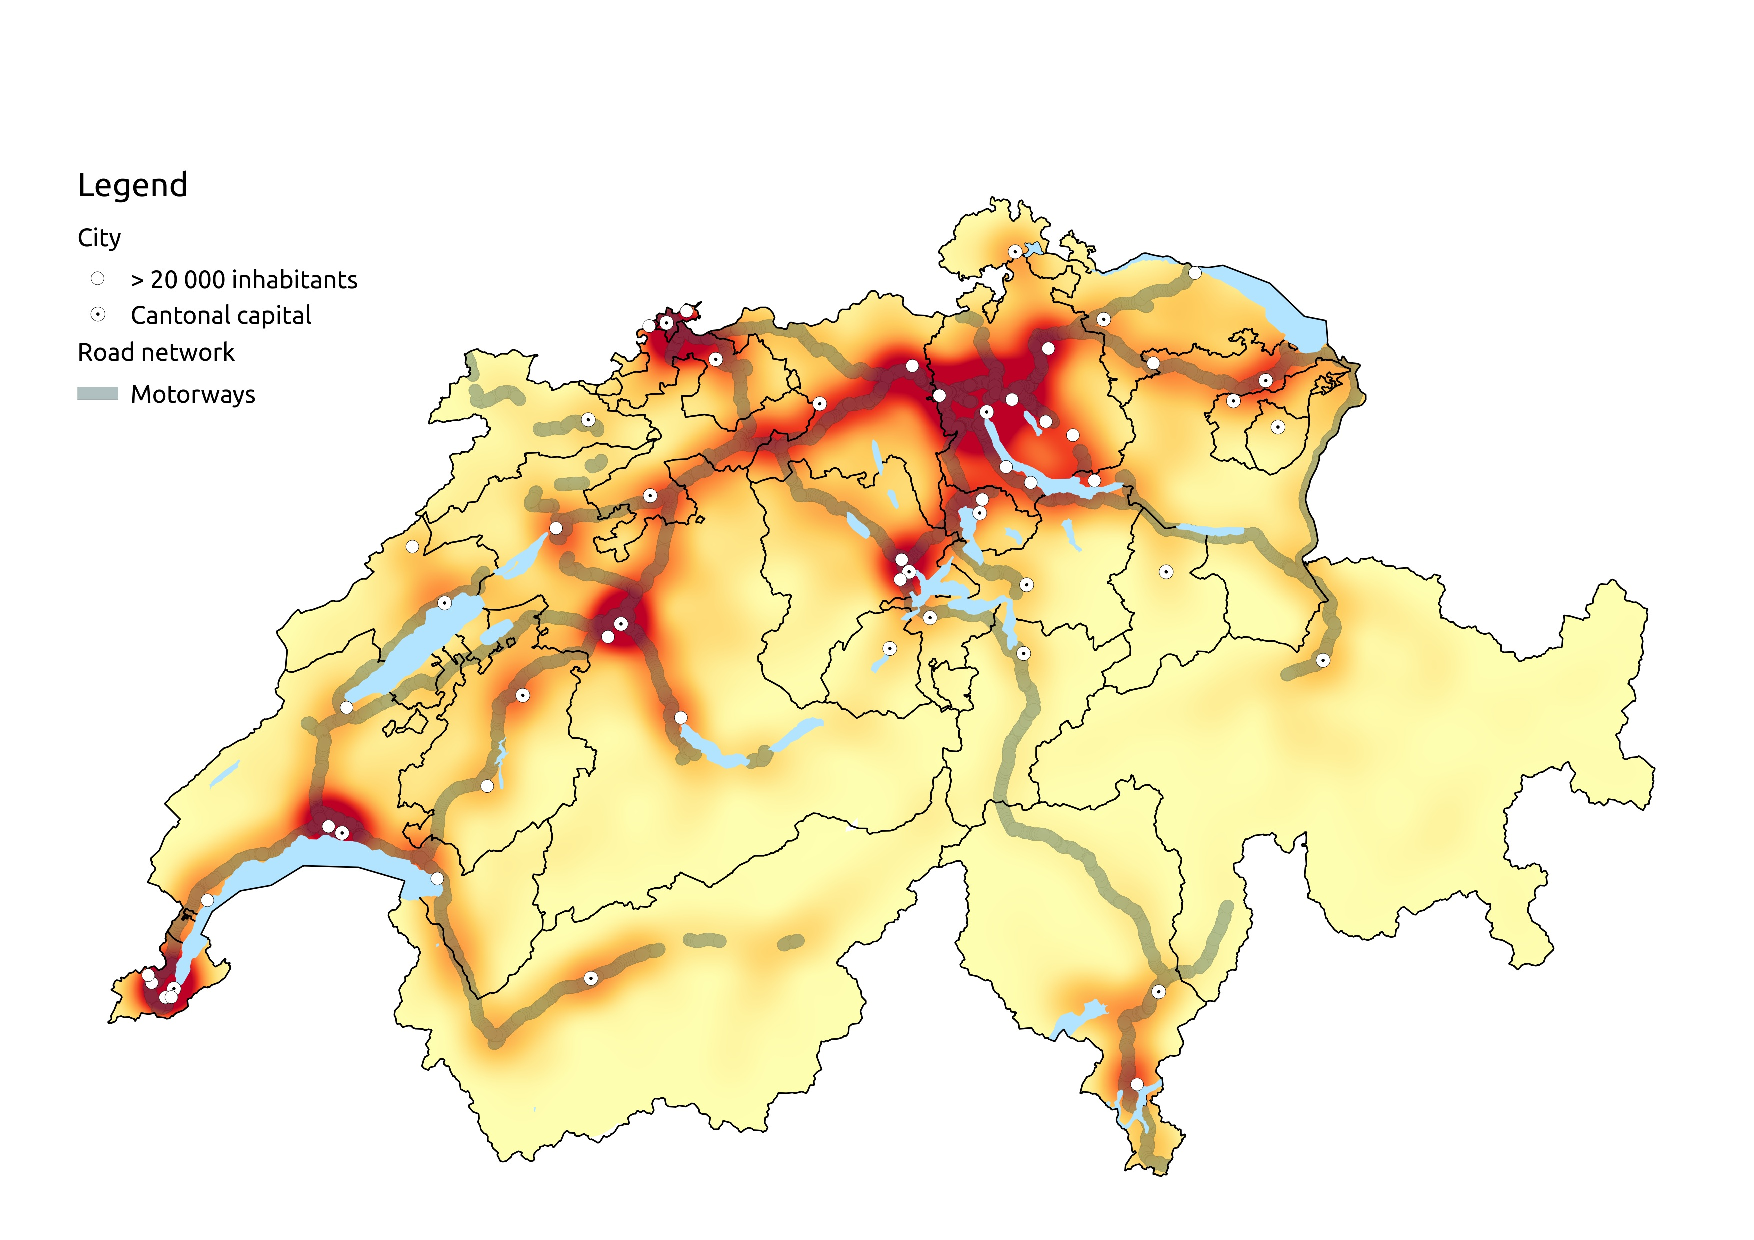
\includegraphics[width=1.0\textwidth, angle=0]{figures/total_emissions_heatmap.pdf}}%
{}

The MATSim computed emissions values are then compared to those estimated by \citet{foen2010pollutants} for 2015.
Since MATSim simulates a single typical workday for 10\% of the entire Swiss population, our values need to be scaled in order to be comparable.
The emissions values are thus multiplied by 10 to account for the population sampling, then by 365 days and finally by an additional scale factor such that the total traveled distance matches the one reported by \citet{foen2010pollutants} for 2015.
\Cref{tab:emissionValueMatsimFoenComparison} shows the total estimated emissions values for both MATSim scenarios and \citet{foen2010pollutants} and \Cref{fig:emissionValueMatsimFoenComparison} plots the percent deviation of the MATSim estimates from the reported 2015 estimates.
The total emission values for all pollutants except PM are within 40\% of the reported values; the values for NO\textsubscript{x}, NO\textsubscript{2} and PM increase with an increase in the diesel engine ownership share.
These deviations are possibly due to the fact that emissions factors depend on the exact type of petrol or diesel engine.
Indeed, in the MATSim model, only one type of petrol and diesel engine is considered, whereas in reality, these are further subdivided into specific subtypes with different emission standards.
Further calibration of the vehicle engine types to the appropriate subtypes could possibly lead to a better fit in emissions values.
Nevertheless, the estimed values coincide with the previously reported values, thereby demonstrating that MATSim provides a reliable means of estimating emission values for pollutants.


\createtable%
{MATSim and FOEN estimated emission value comparison}%
{MATSim and FOEN estimated emission value comparison}%
{\label{tab:emissionValueMatsimFoenComparison}}%
{%
  \begin{tabular}[c]{lrrrrr}
    \toprule
    \multirow{3}{*}{Pollutant} & \multirow{3}{*}{FOEN} & \multicolumn{4}{c}{MATSim} \\ 
    & & \multicolumn{2}{c}{30\% diesel} & \multicolumn{2}{c}{40\% diesel}\\
    & t/a & t/a & \% & t/a & \% \\
    \midrule
	CO\textsubscript{2} (total)  &  10 687 911 &    12 580 738 &	17.71 &	   11 651 538 &		 9.02 \\
	FC         					 &           0 &     4 130 052 &	  --- &     3 823 821 &		  --- \\
	CO         					 &      67 424 &        89 789 &	33.17 &        78 879 &		16.99 \\
	NO\textsubscript{x}     	 &      16 496 &        16 635 &	 0.85 &        20 530 &		24.46 \\
	HC       					 &       9 546 &        10 014 &	 4.90 &         8 952 &		-6.23 \\
	NMHC 					     &       9 037 &         9 467 &	 4.76 &         8 473 &		-6.24 \\
	NO\textsubscript{2}        	 &       4 127 &         4 175 &	 1.15 &         5 441 &		31.83 \\
	PM        					 &         418 &           621 &	48.46 &           764 &		82.67 \\
	SO\textsubscript{2}        	 &          59 &            61 &	 3.06 &            56 &		-4.28 \\
    \bottomrule
  \end{tabular}
}%
{}

\createfigure%
{MATSim and FOEN estimated emission value comparison}%
{MATSim and FOEN estimated emission value comparison}%
{\label{fig:emissionValueMatsimFoenComparison}}%
{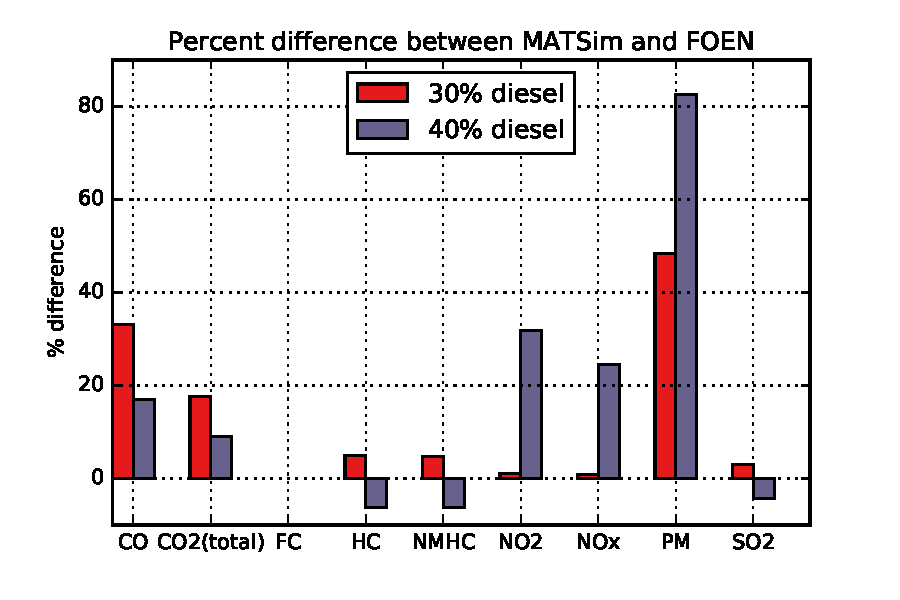
\includegraphics[width=1.0\textwidth, angle=0]{figures/percent_differences.pdf}}%
{}

\subsubsection{Congestion}

Contrary to emissions, congestion and delays caused and experienced cannot directly be estimated from GPS traces alone, since information on how many other drivers were present on the road at that given moment is lacking.
It is precisely for this reason that MATSim is used to estimate congestion throughout a typical workday.
Therefore, it is crucial that the estimated aggregate congestion values are consistent with other previous estimates.
As before, these values are calculated using a 10\% MATSim scenario for Switzerland and are aggregated into hourly time bins per road link.
These estimates are again first analyzed temporally and spatially to assure the plausibility of the output before being compared to the values from \citet{mkinfras2016staukosten}.

The typical total caused and experienced delays pattern per hourly time bin estimated from the MATSim scenario is shown in \Cref{fig:hourlyDelays}.
As was the case for emissions, total delays also expectedly coincide with typical commuter patterns, with fewer delays the early morning and at night, two distinct peaks corresponding to morning and evening rush-hour and midrange values at midday.
One notices in \Cref{fig:hourlyDelays} that there are higher caused delays than experienced delays at the start of the peaks whereas the opposite is true towards the end of the peaks, a manifestation of the fact that delays first need to be caused before they can be experienced.
Nonetheless, the total duration of both caused and experienced delays are equal and sum up to just under 250 000 hours.


\createfigure%
{Hourly total caused and experienced delays for Switzerland}%
{Hourly total caused and experienced delays for Switzerland}%
{\label{fig:hourlyDelays}}%
{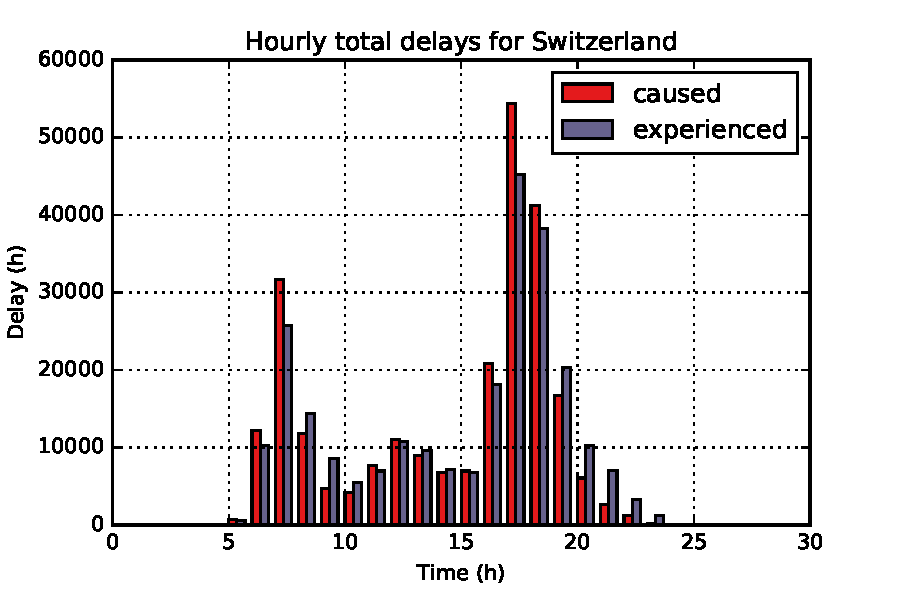
\includegraphics[width=0.8\textwidth,
angle=0]{figures/hourly_delays.pdf}}%
{}

\Cref{fig:spatialDelays} shows the spatial distribution of the total daily experienced delays over entire Switzerland.
The heatmap is generated by summing the total experienced delays with a 1 km radius around each point.
Following an anogolous reasoning as for emissions, longer delay times are observed in and around larger cities and within highly populated cantons, where more people live and commute to.

\createfigure%
{Spatial distribution of total experienced delays in Switzerland}%
{Spatial distribution of total experienced delays in Switzerland}%
{\label{fig:spatialDelays}}%
{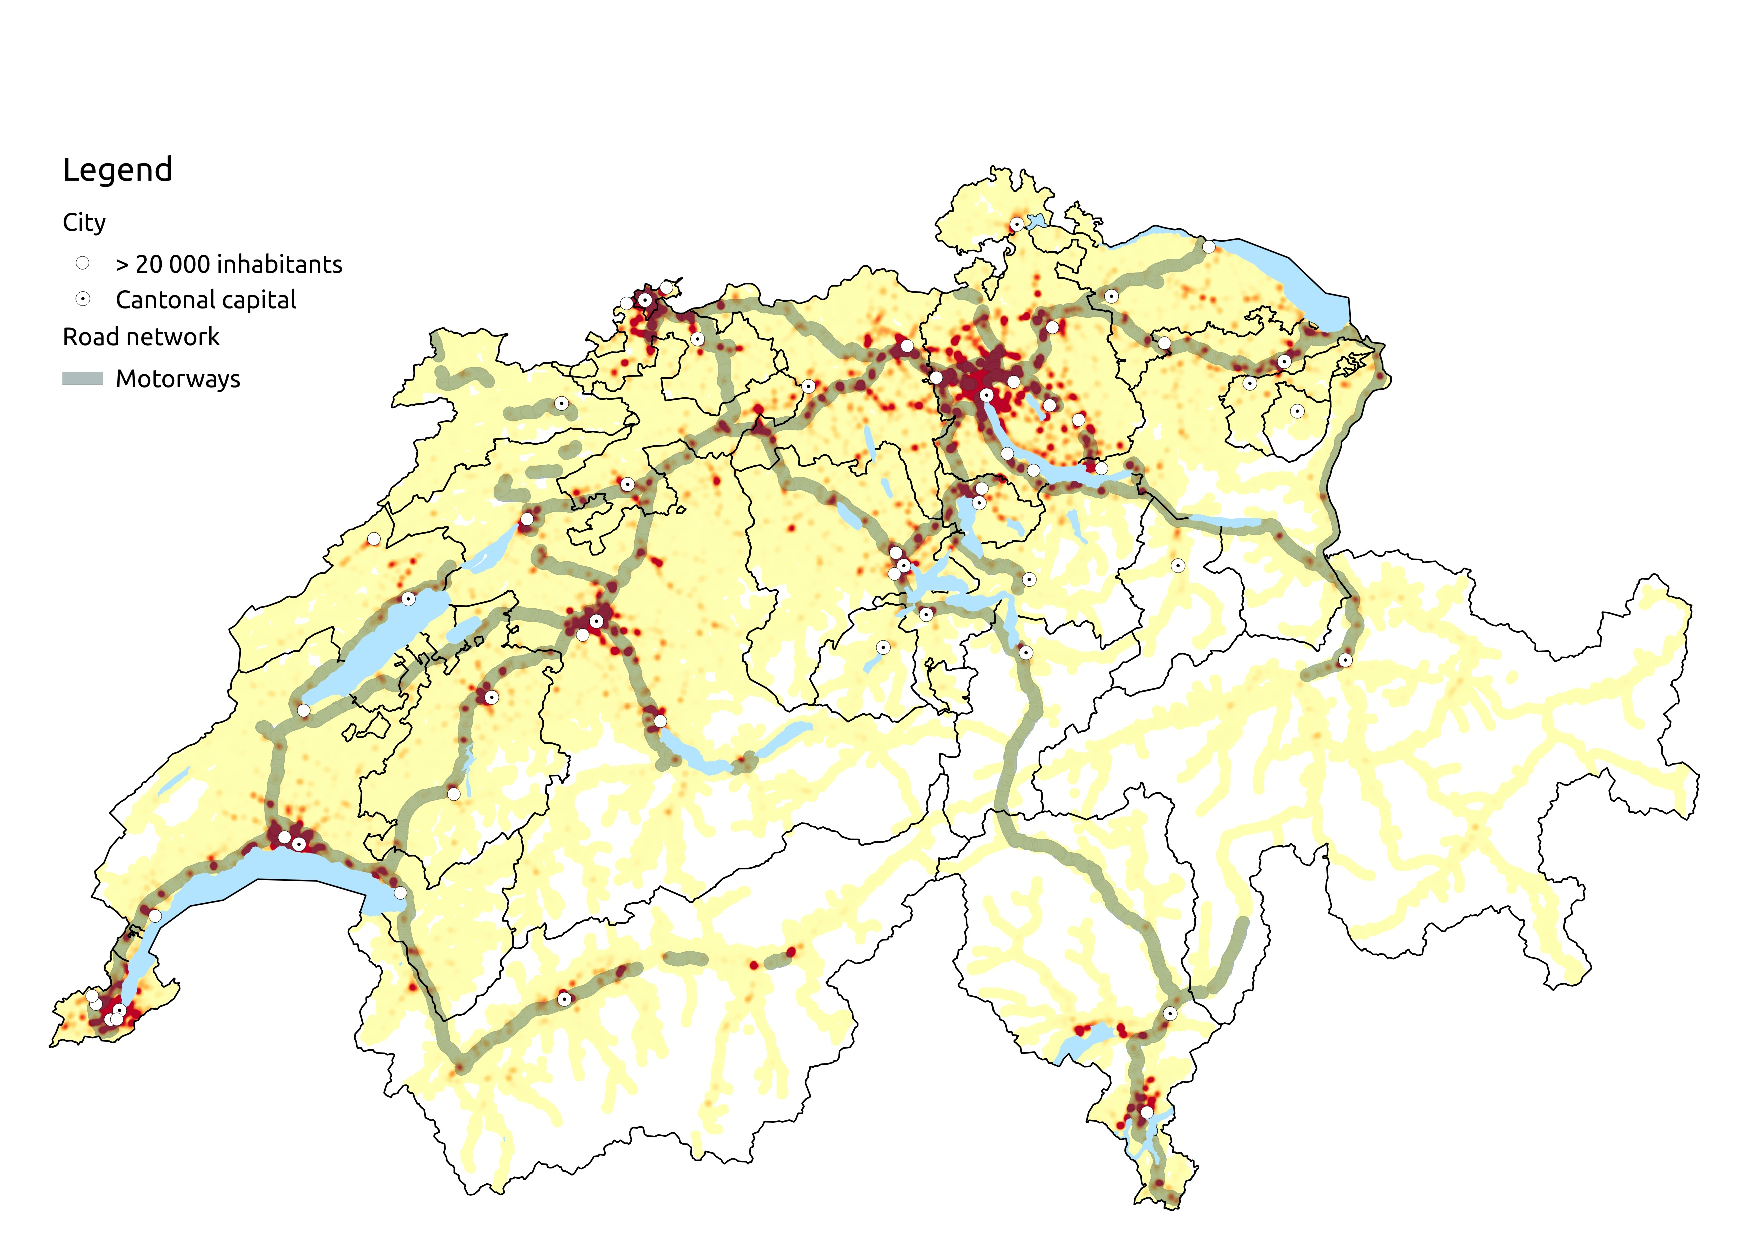
\includegraphics[width=1.0\textwidth, angle=0]{figures/total_delays_heatmap.pdf}}%
{}

The MATSim computed delay values are then compared to those calculated by \citet{mkinfras2016staukosten}.
The same scaling operations are performed as in the case of emissions: multiplication by 10 to account for the population sampling, then by 365 days and finally by an additional scale factor such that the total traveled distance matches the one reported by \citet{mkinfras2016staukosten} for 2014.
The values are reported in \Cref{tab:delayValueComparison}.


\createtable%
{MATSim and Infras / MK Consulting congestion comparison}%
{MATSim and Infras / MK Consulting congestion comparison}%
{\label{tab:delayValueComparison}}%
{%
  \begin{tabular}[c]{lrrr}
    \toprule
    Road type & MK/Infras (Mveh-h/a) & MATSim (Mveh-h/a) & \%  \\ 
    \midrule
    Motorway      & 16.62 &    8.33 &  -49.89 \\
    Non-motorway  & 11.23 &   95.00 &  745.98 \\
    Total &         27.85 &  103.33 &  271.03 \\
    \bottomrule
  \end{tabular}
}%
{}

The total vehicle hour delay per year values are estimated to be much higher in MATSim than in \citet{mkinfras2016staukosten}.
However, the authors do indeed state that they have taken an "at-least" approach in estimating delays and that the values for non-motorway segments are highly underestimated.
On the other hand, our model only simulates passengers vehicles.
Therefore, it neither accounts for the effects of the interaction of cars with trucks on motorways nor does it captures extraordinary circumstances such as accidents and holiday traffic which could increase the vehicle hours of delay.
A combination of these effects could be the underlying cause of the deviation between the estimates and should be further investigated.


\subsection{Green Class Emission Reductions}
A core component of the Green Class pilot project was the availability of an electric car to subscribers. These cars were covered by renewable energy certificates, negating the need to consider the energy generation makeup in calculating the emissions reductions. For the analysis, it is assumed that for trips performed with an electric vehicle, the driving style, route choice and trip timing is independent of the choice of vehicle. Additionally, the possibility that the availability of electric vehicles generated mode shifts away from other modes (i.e. train travel, cycling or car sharing) is excluded. 
The effects of having an additional vehicle in multi-car households are also excluded. 

\createtable%
{Reduction in emissions due to the availability of an electric vehicle}%
{Reduction in emissions due to the availability of an electric vehicle}%
{\label{tab:reduction_summary}}%
{%
\begin{tabular}{rrrr}
  \hline
 & Car & Ecar & Reduction (\%) \\ 
  \hline
CO (kg) & 45.51 & 37.26 & 45.02 \\ 
  CO\textsubscript{2} (T) & 11.32 & 8.97 & 44.20 \\ 
  FC (T) & 3.60 & 2.85 & 44.20 \\ 
  HC (kg) & 4.53 & 3.68 & 44.80 \\ 
  NMHC (kg) & 4.27 & 3.46 & 44.80 \\ 
  NO\textsubscript{x} (kg) & 24.18 & 19.34 & 44.43 \\ 
  NO\textsubscript{2} (kg) & 4.12 & 3.28 & 44.37 \\ 
  PM (kg) & 1.22 & 0.97 & 44.29 \\ 
  SO\textsubscript{2} (kg) & 0.06 & 0.05 & 44.20 \\ 
   \hline
\end{tabular}
}%
{}

\Cref{tab:reduction_summary} presents the reduction of various emissions over the course of the program due to the availability of the E-car. 
A clear immediate reduction in daily CO\textsubscript{2} emissions is observed in \Cref{fig:green-class-reduction}. 
Overall, a reduction of 30\% can be observed with respect to the pre-Ecar period. 
There are however some noticeable outliers, particularly April 1\textsuperscript{st}, 2017. 
During the course of the pilot program, subscribers had unrestricted access to both their personal vehicle and the provided electric vehicle. 
As such, on days where many subscribers choose to use their personal vehicles, emissions will naturally be nearer to the pre-program levels. 
A particular reason for such a choice would be public holidays where many subscribers are likely to want to travel further than what the range of the electric vehicle permits.

\createfigure%
{Percentage of pre-electric vehicle CO\textsubscript{2} produced per day. EV's were provided on January 16, 2017. }%
{Percentage of pre-electric vehicle CO\textsubscript{2} produced per day. EV's were provided on January 16, 2017. }%
{\label{fig:green-class-reduction}}%
{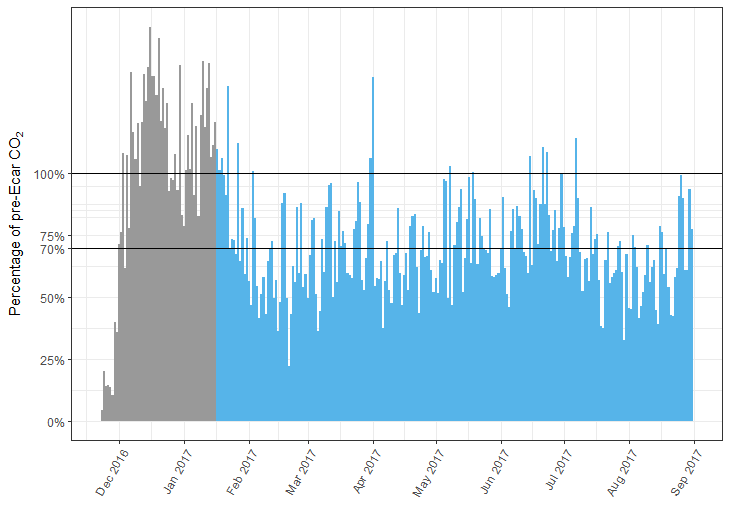
\includegraphics[width=1.0\textwidth, angle=0]{figures/green_class_pollutant_reductions_daily}}%
{}

The 139 subscribers were not representative of the general population, due to the high cost (12,200 CHF) and selective nature of the pilot program.
Nevertheless, these results demonstrate the environmental benefit of having an electric vehicle, and that persons with access to both will significantly reduce their emissions by using the electric vehicle.

%%%%%%TODO: add a comparison of congestion experienced vs congsetion caused for Green Class drivers